% This is samplepaper.tex, a sample chapter demonstrating the
% LLNCS macro package for Springer Computer Science proceedings;
% Version 2.20 of 2017/10/04
%
\documentclass[runningheads]{llncs}
%
\usepackage{graphicx}
\usepackage{hyperref}
% Used for displaying a sample figure. If possible, figure files should
% be included in EPS format.
%
% If you use the hyperref package, please uncomment the following line
% to display URLs in blue roman font according to Springer's eBook style:
\renewcommand\UrlFont{\color{blue}\rmfamily}
\usepackage{cite}
\usepackage{algorithm}
\usepackage{algorithmic}

\usepackage{changepage}
\usepackage{comment}
\usepackage[title]{appendix}
\usepackage{enumitem}
\usepackage{caption}
\usepackage[font=scriptsize]{subcaption}
\usepackage{color} % added by Bayzid
\newcommand{\commentA}[1]{{\color{red} #1}}
\newcommand{\commentM}[1]{{\color{blue} #1}}
\usepackage{subcaption}
\renewcommand{\algorithmiccomment}[1]{~{\scriptsize\ttfamily{/*#1*/}}}
\usepackage{enumitem}

%to squeeze space between sections, subsections and subsubsections
\makeatletter
\renewcommand\section{\@startsection{section}{1}{\z@}%
	{-8\p@ \@plus -4\p@ \@minus -4\p@}%
	{6\p@ \@plus 4\p@ \@minus 4\p@}%
	{\normalfont\large\bfseries\boldmath
		\rightskip=\z@ \@plus 8em\pretolerance=10000 }}
\renewcommand\subsection{\@startsection{subsection}{2}{\z@}%
	{-8\p@ \@plus -4\p@ \@minus -4\p@}%
	{6\p@ \@plus 4\p@ \@minus 4\p@}%
	{\normalfont\normalsize\bfseries\boldmath
		\rightskip=\z@ \@plus 8em\pretolerance=10000 }}
\renewcommand\subsubsection{\@startsection{subsubsection}{3}{\z@}%
	{-4\p@ \@plus -4\p@ \@minus -4\p@}%
	{-1.5em \@plus -0.22em \@minus -0.1em}%
	{\normalfont\normalsize\bfseries\boldmath}}
\makeatother
%\captionsetup{belowskip=-10pt}

\begin{document}
%
\title{Improving accuracy of Estimated Species Tree Through Multi-objective Optimization}
\author{}
\institute{}
%
\maketitle              % typeset the header of the contribution
%

\begin{abstract}
The abstract should briefly summarize the contents of the paper in
15--250 words.

\keywords{Phylogenomics  \and Multi-objective
optimization \and Genetic Algorithm.}
\end{abstract} 
\section{Introduction}
\label{sec:intro}
Unveiling the mechanisms that control gene expression is a major challenge in biology. One of the most important tasks in this challenge is to identify \textbf{conserved regions} in deoxyribonucleic acid (DNA) for transcription factors. These \textit{short conserved regions} are known as motifs. 
\section{Related Work}
\label{sec:literature} 
\section{Problem Desscription}
\label{sec:problem}

\section{Methods}
\label{sec:method}
\section{Results}
\label{sec:results}

\begin{figure}[!htbp]
	%\scriptsize
	\centering
	\begin{adjustwidth}{-1cm}{-1cm}
		\begin{subfigure}[b]{0.4\textwidth}
			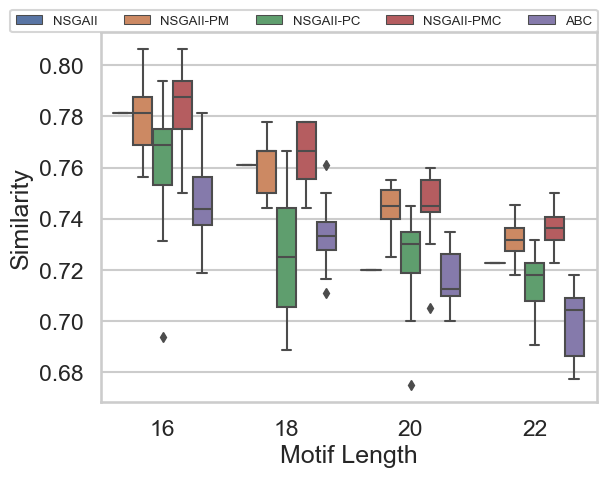
\includegraphics[width=\textwidth]{Figure/hm03_all_boxplot}
			\caption{hm03}
			%\label{fig:con_pr06}
		\end{subfigure}%
		\begin{subfigure}[b]{0.4\textwidth}
			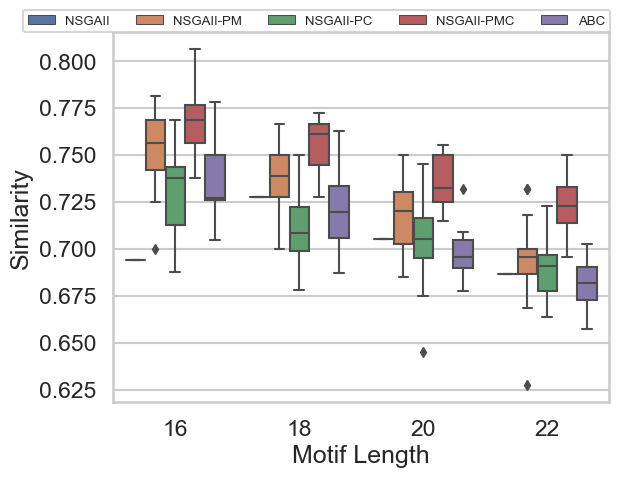
\includegraphics[width=\textwidth]{Figure/hm09g_all_boxplot}
			\caption{hm09g}
			%\label{fig:con_pr07}
		\end{subfigure}%
		\begin{subfigure}[b]{0.4\textwidth}
			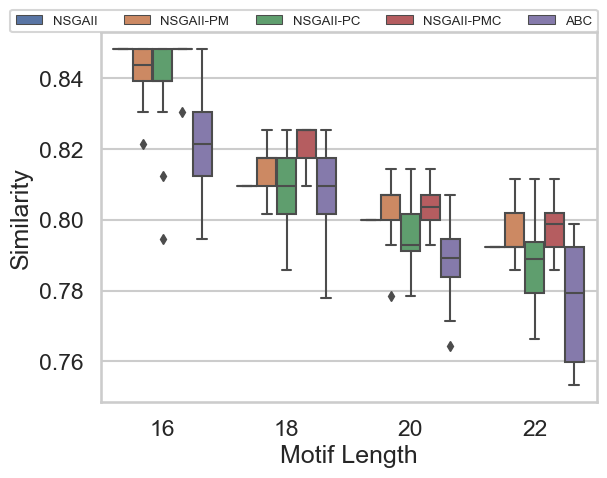
\includegraphics[width=\textwidth]{Figure/yst04r_all_boxplot}
			\caption{yst04r}
			%\label{fig:con_pr09}
		\end{subfigure}    
		\begin{subfigure}[b]{0.4\textwidth}
			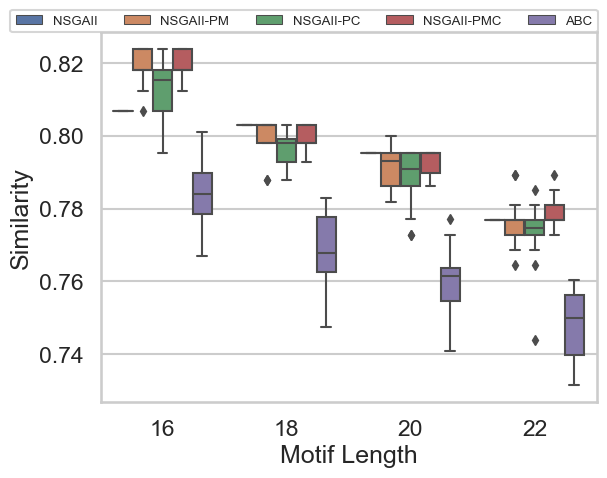
\includegraphics[width=\textwidth]{Figure/yst08r_all_boxplot}
			\caption{yst08r}
			%\label{fig:con_pr06}
		\end{subfigure}%
		\begin{subfigure}[b]{0.4\textwidth}
			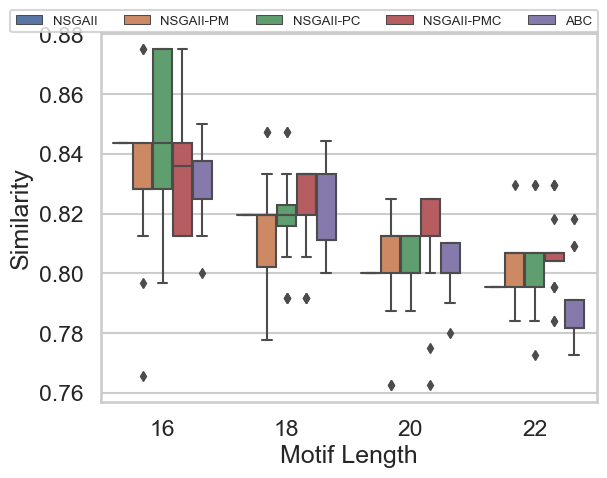
\includegraphics[width=\textwidth]{Figure/dm01g_all_boxplot}
			\caption{dm01g}
			%\label{fig:con_pr07}
		\end{subfigure}%
		\begin{subfigure}[b]{0.4\textwidth}
			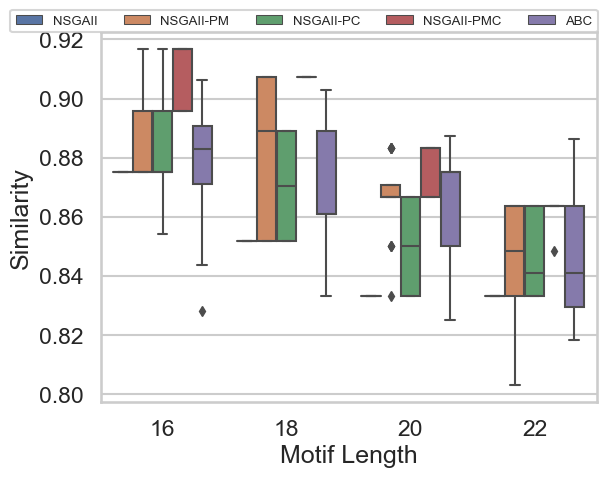
\includegraphics[width=\textwidth]{Figure/dm03g_all_boxplot}
			\caption{dm03g}
			%\label{fig:con_pr09}
		\end{subfigure}
		\caption{Similarity score achieved by ABC and four NSGAII variants on six datasets. }
		\label{fig:gen_wise_correlation}
	\end{adjustwidth}
\end{figure}
\section{Conclusion}
\label{sec:conclusion}



%
% ---- Bibliography ----
%
% BibTeX users should specify bibliography style 'splncs04'.
% References will then be sorted and formatted in the correct style.
%
\bibliographystyle{splncs04}
\bibliography{main_bib}
\end{document}
